\chapter{Metodologia}
\label{cap3}

\section{Resumo}

\paragraph{} As seções a seguir trazem detalhes quanto a estrutura técnica do projeto. Portanto, a Figura \ref{fig:100} mostra uma noção geral de como as estrutras se conectam.

\begin{figure}[h]
    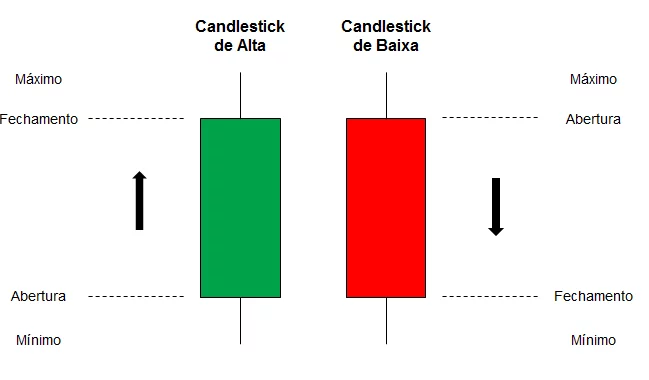
\includegraphics[scale=0.50]{candlestick.png}
    \centering
    \caption{Leitura de um gráfico de \textit{candlestick} \cite{candlestick}}
    \label{fig:100}
\end{figure}

\paragraph{} Primeiro, tem-se início a etapa de pré-processamento de dados,  ...

\section{Pré-Processamento}

\subsection{Arquivo de Configuração}
\paragraph{} Falar motivação do arquivo; Print de exemplo; Apontar para subsection de lista de parâmetros; Possibilidade de rodar várias simulações.

\subsection{Coleta de Dados}
\paragraph{} yfinance; Problema com proventos; Normalização de proventos do preço das ações.

\subsection{Armazenamento de Dados}
\paragraph{} Banco de dados; Criação de Candles semanais.

\subsection{Geração de Features de Uso Geral}
\paragraph{} Quais features; Cuidados com não-causalidade.


\section{Simulação de Estratégia}

\subsection{Estrutura}
\paragraph{} Carteira com N ativos de datas distintas; Regra de 3 para 1 entre stop e alvo; 1 operação por ativo.

\subsection{Premissas}
\paragraph{} Compra na abertura do merdado; Sem venda no dia da compra; Prioridades durante venda (stop primeiro).

\subsection{Período Máximo de Dias por Operação}
\paragraph{} Motivação da escolha dos 45 dias; Gráfico entre ABEV e MGLU.

\subsection{Gerenciamento de Risco}
\paragraph{} Coeficiente de Risco-Capital

\subsection{Risco de Entrada por Operação}
\paragraph{} Cálculo do risco mínimo; Cálculo do risco Máximo.

\subsection{Descanso por Tendência de Baixa}
\paragraph{}

\subsection{Descanso por Identificação de Crises}
\paragraph{}

\subsection{Lista de Parâmetros de Configuração}
\paragraph{} Lista todos e explicar o que fazem.

\subsection{Ensaios Paralelos}
\paragraph{} Parâmetros que estão implementados e não trouxeram resultados expressivos.



\section{Otimizações de Gerenciamento de Carteira}

\subsection{Normalização por Frequência de Operações}
\paragraph{}

\subsection{Controle Proporcional para Uso de Capital}
\paragraph{}

\subsection{Compensação por Lucratividade}
\paragraph{}



\section{Criação de Modelos}

\subsection{Resumo}
\paragraph{}

\subsection{\textit{Feature Selection}}
\paragraph{}

\subsection{Geração de \textit{Datasets}}
\paragraph{}

\subsection{\textit{Walk Forward Optimization}}
\paragraph{}

\subsection{Critérios de Escolha}
\paragraph{}


\section{Análise de Resultados}
\paragraph{} Dashboard; Baseline